% "{'classe':('PSI'),'chapitre':'chs_leq','type':('td'),'titre':'Tour de la terreur', 'source':'Vuibert','comp':('B2-15'),'corrige':False}"
%\setchapterimage{bandeau}
\chapter*{Application \arabic{cptApplication} :\\ 
Tour de la terreur -- \ifprof Corrigé \else Sujet \fi}
\addcontentsline{toc}{section}{Application \arabic{cptApplication} : Tour de la terreur -- \ifprof Corrigé \else Sujet \fi}

\iflivret \stepcounter{cptApplication} \else
\ifprof  \stepcounter{cptApplication} \else \fi
\fi

\setcounter{question}{0}
\marginnote{D'après Livre Ed. Vuibert.}
\marginnote[1cm]{
\UPSTIcompetence[2]{B2-15}
}
%\begin{marginfigure}
%\centering
%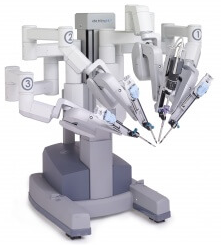
\includegraphics[width=4cm]{fig_00}
%\end{marginfigure}




\begin{marginfigure}
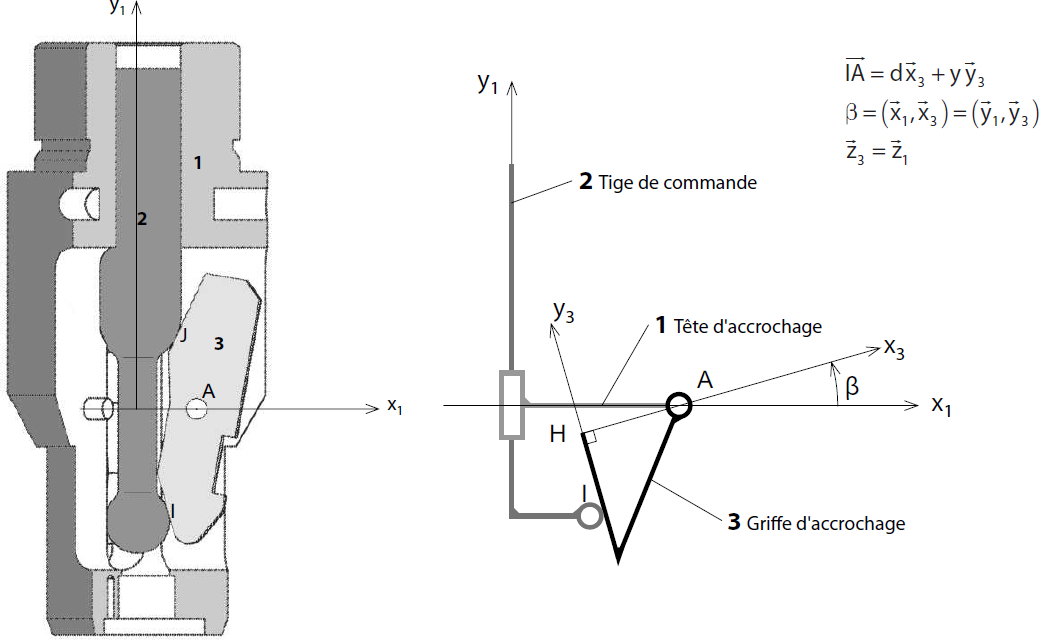
\includegraphics[width=\linewidth]{fig_01}

\caption{Guidage de l'ascenseur.}
\end{marginfigure} 


La Tour de la terreur du parc Walt Disney Studios propose aux visiteurs d'entrer dans une tour et d'effectuer une chute de 13 étages dans un ascenseur.
L'ascenseur est guidé en translation sur deux rails par 12 galets répartis sur 4 systèmes de guidage.


%\begin{figure}[!ht]
%\centering
%\begin{tikzpicture}
%
%\node at (0,0) {\includegraphics[height=3.5cm]{\pathfig/tour1a_nb}};
%\node at (4,0) {\includegraphics[height=3.5cm]{\pathfig/tour1b_nb}};
%%\draw[gray!50] (-3,3) grid[step=1mm] (6,-2);
%%\draw[gray!90] (-3,3) grid[step=5mm] (6,-2);
%%\node {$\times$};
%
%\node[fill=white,left] at (-2.2,1) {\footnotesize{Galets}}; 
%\node[fill=white,left] at (1,-2.3) {\footnotesize{Guidage en $A$}}; 
%\end{tikzpicture}
%\caption{Tour de la terreur et guidage de l'ascenseur.}
%\end{figure}

%\begin{center}
%\begin{tabular}{cc}
%\includegraphics[height=4.5cm]{\pathfig/tour1a}&
%\includegraphics[height=4.5cm]{\pathfig/tour1b}
%\end{tabular}
%\end{center}

\subsection*{Cahier des charges\\}

Le diagramme des exigences partiel de la Tour de la terreur est donné figure suivante.


\begin{figure}[!h]
\centering
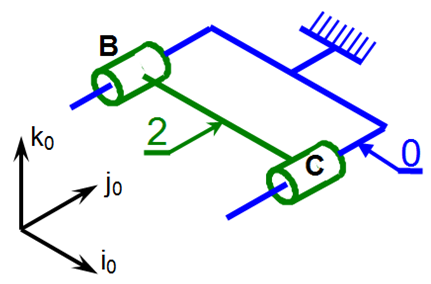
\includegraphics[width=.8\linewidth]{fig_02}

\caption{Diagramme des exigences partiel.}
\end{figure}

%\begin{figure}[!ht]
%\centering
%%\includegraphics{\pathfig/Exigences_Tour}
%\includestandalone[width=.8\linewidth]{\pathfig/Diagramme_exigences_tour}
%\caption{Diagramme des exigences partiel.}
%\label{reqtour}
%\end{figure}

\begin{obj}
L'objectif est d'analyser différentes liaisons en parallèle ou en série de la Tour de la terreur afin de valider l'exigence de précision du guidage lors de la descente.
\end{obj}


%\textcolor{red}{DV : mettre des dimensions h en hauteur et L en largeur}


\begin{figure}[!h]
\centering
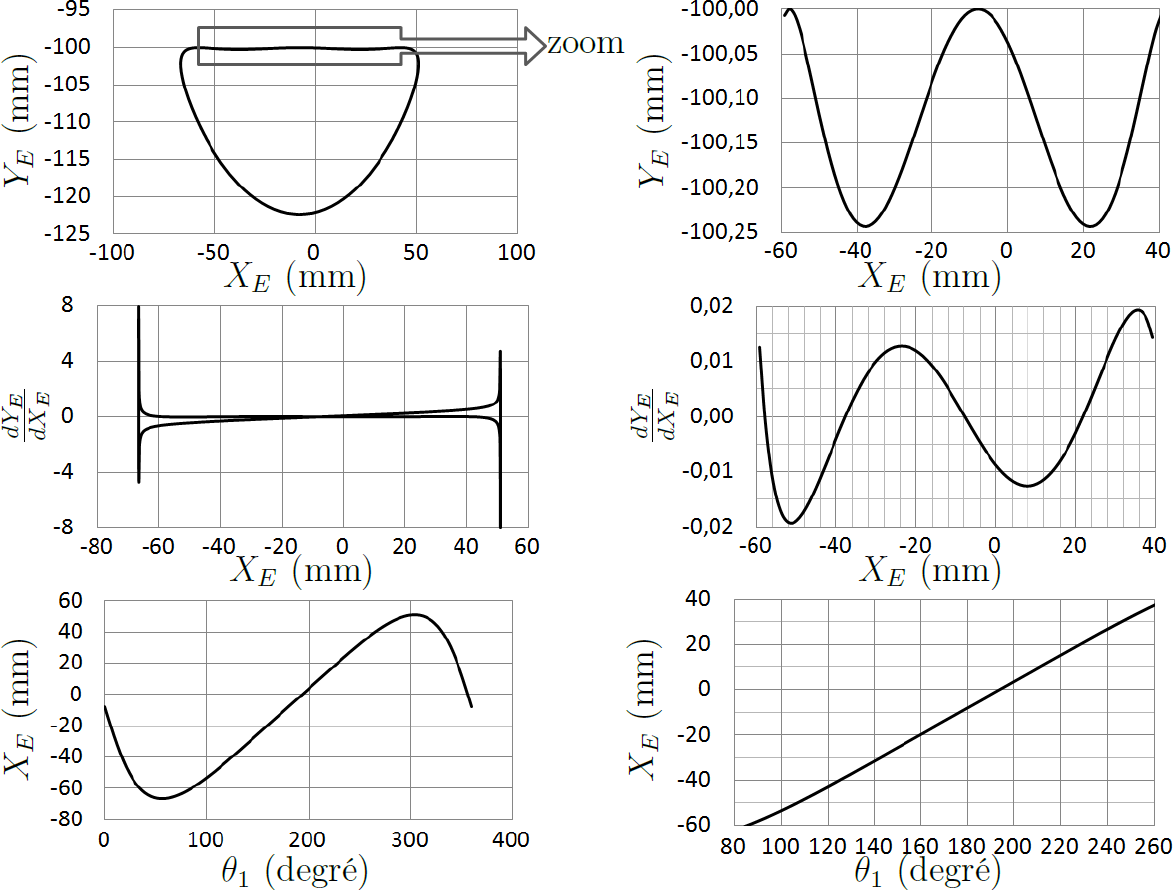
\includegraphics[width=.8\linewidth]{fig_03}

\caption{Modélisation de la Tour.}
\end{figure}

%
%\bigskip
%\noindent
%%\includegraphics[height=7cm]{\pathfig/tour2a.pdf}\hfill
%\includegraphics[height=7cm]{\pathfig/tour2a.png}\hfill
%\begin{tikzpicture}
%%\node (i) {\includegraphics[height=7cm]{\pathfig/tour2b.pdf}};
%\node (i) {\includegraphics[height=7cm]{\pathfig/tour2b.png}};
%\coordinate (o) at (i.south west);
%\draw[->,>=latex] (o) -- ++(1,0) node[right] {$\vect y$};
%\draw[->,>=latex] (o) node[below left] {$O$} -- ++(0,1) node[left] {$\vect z$};
%\draw [latex-latex] (2.5,-1.8) --++(0,2.4) node [right,midway] {$h$};
%\draw [latex-latex] (-1.1,-1.8) --++(3.3,0) node [above,midway] {$L$};
%\end{tikzpicture}
%\captionof{figure}{Modélisation de la Tour.}
%
%
%\piccaption{Association en série d'une liaison pivot et d'une liaison  ponctuelle.\label{SeriePivotPonctuelle}}
%\parpic[r]{\includestandalone{\pathfig/PonctuelleEtPivotSerie}}

On modélise chaque contact entre un galet et le rail par une liaison 
ponctuelle.  On modélise chaque liaison entre un galet et la cabine par une liaison pivot.

Afin de simplifier l'étude, nous nous intéressons d'abord à la liaison équivalente à une liaison pivot en série avec une liaison ponctuelle (liaison réalisée entre la cabine et un rail par l'intermédiaire d'un seul galet).

\begin{marginfigure}[-2cm]
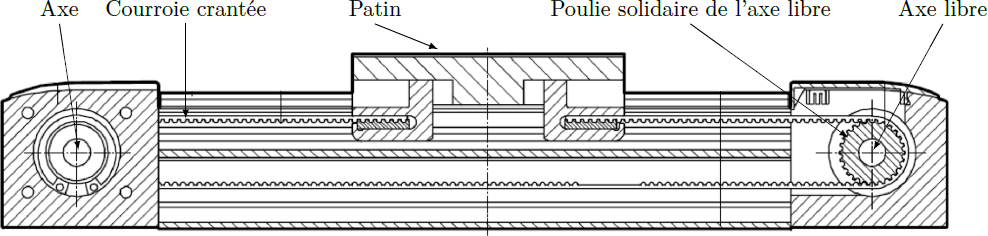
\includegraphics[width=.8\linewidth]{fig_04}

\caption{Association en série d'une liaison pivot et d'une liaison  ponctuelle.}
\end{marginfigure}

%
%%\begin{figure}[htbp!]
%%%\includegraphics[width=0.3\textwidth]{\pathfig/PonctuelleEtPivotSerie.png}
%%\caption{}
%%\label{SeriePivotPonctuelle}
%%\end{figure}
%\vspace{1.5cm}}

%\question{En utilisant le modèle de la figure précédente,  montrer que l'association en série d'une ponctuelle de normale $\vect{n}$ et d'une liaison pivot d'axe $\vect{z}$ est équivalente à une liaison ponctuelle de normale $\vect{n}$.}

\ifcolle
\question{Proposer un graphe des liaisons et proposer une méthode permettant de déterminer la liaison équivalente entre la cabine et le sol.}
\else
\fi

\question{En utilisant le modèle de la figure précédente, déterminer la liaison équivalente à l'association en série d'une ponctuelle de normale $\vect{n}$ et d'une liaison pivot d'axe $\vect{z}$.}

Dans la suite, nous considérerons cette simplification pour tous les galets.

\question{Proposer un graphe des liaisons faisant intervenir les modèles des 12 galets entre le rail et l'ascenseur.}

\question{Donner le torseur cinématique d'une liaison ponctuelle ou sphère-plan en précisant le point d'écriture et la base.}

%\question{Montrer que l'association de trois liaisons ponctuelles en parallèle au niveau d'un guidage ($A$, $B$, $C$ ou $D$) est équivalente à une liaison sphère-cylindre dont on précisera les caractéristiques.}

\question{Donner la liaison équivalente à l'association de trois liaisons ponctuelles en parallèle au niveau d'un guidage ($A$, $B$, $C$ ou $D$).}

\question{Montrer que l'association en parallèle de deux liaisons sphère-cylindre de même axe est équivalente à une liaison pivot glissant.}

%\newpage
%\enlargethispage{\baselineskip}

\question{Conclure sur la liaison équivalente entre la cabine et le rail compte tenu des résultats précédents.}

\question{Pourquoi utilise-t-on cette solution pour guider la cabine de l'ascenseur ?}




